\chapter{Connectivity}
	A (non empty) graph is \textit{connected} when there is a path between every pair of vertices. In a connected graph, there are no unreachable vertices. A graph that is not connected is \textit{disconnected}.\\

	A graph with just one vertex is connected. An edgeless graph with two or more vertices is disconnected.\\
	
	A graph $G$ is \textit{$k$-connected} if $|V(G)| \geq k + 1$ and $\nexists X \subseteq V$ with $|X| \leq k-1$ such that $G-X$ is disconnected.\\
	
	The \textit{vertex connectivity} of $G$ is the maximum $k$ so that $G$ is $k$-connected.\\
	
	A vertex $v \in V(G)$ is a \textit{cut vertex} of a connected graph $G$ is $G - \{ v \}$  is not connected.

	\section{2-Connected graphs and subgraphs}
		There are at least 3 vertices and there isn't any cut vertex.\\
		
		A \textit{block} of a graph $G$ is an induced subgraph $B$ of $G$ such that $B$ is connected and has no cut vertex and $B$ is maximal with this property.\\
		
		A block $B$ can be:
			\begin{itemize}
				\item a \textit{bridge}: $B = \{x,y\}$ with $xy \in E(G)$ and $G - xy$ is disconnected.
				\item a 2-connected induced subgraph: if $|B| \geq 3$, and $B$ is maximal with this property.
				\item a single vertex: $|B| = 1$, when $G$ has a singleton component.
			\end{itemize}
			
		Let us make an observation: if $B_1$ and $B_2$ are two distinct blocks, then they have at most one vertex in common, and if they do then that vertex is a cut vertex of $G$.\\
		
		And another: let's make a bipartite graph with, on the one hand, the blocks and on the other hand, the cut vertices.\\

                Blocks define a tree structure (no cycle).

		\subsection{Theorem: ear decomposition of 2-connected graphs}
		Let $G$ be 2-connected $\iff G$ can be built starting with a cycle and iteratively adding ears.\\
		
		\begin{figure}
			\center
			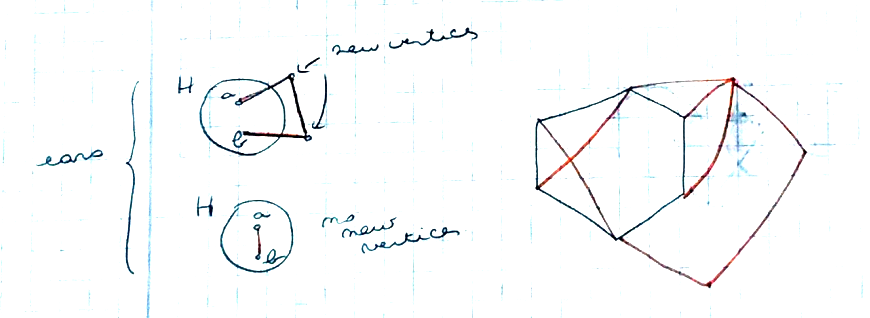
\includegraphics{img/3-1}
		\end{figure}
		Proof: 
		\begin{enumerate}
			\item $\impliedby$ OK
			\item $\implies$ Let $H \subseteq G$ be a subgraph of $G$ that can be constructed by the procedure and maximal with this property. Note that $H$ exists because $G$ has at least one subgraph that can be constructed, namely a cycle (since $G$ is 2-connected). We want to show $H = G$. Suppose not (pf by contradiction): 
				\begin{enumerate} 
					\item $V(H) = V(G) \implies \exists e \in E(G) - E(H)$ then we could have added $e$ to $H$, contradicting the maximality of $H$.
					\item $V(H) \neq V(G)$. We connect a vertex from an ear to a vertex from the cycle $H$. Since $G$ is connected, $\exists ab \in E(G)$ with $a \in V(H), b \notin V(H)$. Since $G$ is 2-connected, $G-a$ is connected, so there is a path $P$ linking $b$ to $V(H) - \{a\}$ in $G- a$, hence we could have added the ear $P + ab$ to $H \rightarrow$ contradiction. 
				\end{enumerate}
		\end{enumerate}
		
		
	\section{The structure of 3-connected graphs}

		\subsection{Lemma (Tutte)}
		\textit{If $G$ is 3-connected and $|V(G)| \geq 5$, then $\exists e \in E (G)$ such that $G / e$ is still 3-connected.}\\
		
		Note that $G / e$ is the graph $G$ following the contraction of the edge $e$.\\
		
		Proof: by contradiction, assume there is no such edge.
		\begin{enumerate}
			\item Consider any edge $xy \in E(G)$. Now $H := G / xy$ is not 3-connected, thus there is a subset $S$ of vertices of $H$ with $|S| \leq 2$ so that $H - S$ is not connected. 
			\item Observation: if $v_{xy}$ denotes the vertex of $H$ resulting from the contraction of $xy$, then we must have $v_{xy} \in S$, because without otherwise $S$ would also be a cut set of $G$ of size $\leq 2$.
			\item On the  other hand, if $S'$ is obtained from $S$ by replacing $v_{xy}$ with $x,y$ then $S'$ is a cut set of $G \implies |S'| \geq 3 \implies |S| = 2$.
		\end{enumerate}
		
		Any 3-connected graph can be contracted to $K_4$ by iteratively contracting edges, in such a way that each intermediate state remains 3-connected.
		
		
	\section{Menger's theorem}
		\textit{Let $G = (V,E)$ be a graph and $A, B \subseteq V$. Then the minimum number of vertices separating $A$ from $B$ in $G$ is equal to the maximum number of disjoint $A-B$ paths in $G$.\\}

		\begin{enumerate}
			\item Proof $\impliedby$: Take distinct $a ,b \in V(G)$. Since there are $k$ independent $a-b$ paths and at least $k-1$ of these have at least one internal vertex, $G$ has $\geq 2 + k - 1 = k + 1$ vertices. Moreover, there is no $Y \subseteq V(G)$ of size less than $k$ such that $G - Y$ is not connected, because o/w: pick $a,b$ in distinct components of $G - Y$. Every $a-b$ path goes through $Y$, hence there cannot be $k$ independent $a-b$ paths.
			\item Proof $\implies$: consider two distinct vertices $a,b \in V(G)$. 
		\begin{enumerate}
		\item{Case 1: $ab \notin E(G)$}
		Let $A := N(a)$ and $B := N(b)$.
		If there are $k$ disjoint $A-B$ paths then there are $k$ such paths avoiding $a,b$ and we see that there are $k$ independent paths in $G$.  Observe $|A| \geq k$ and $|B| \geq k$.\\
		
		If $\not{\exists} k$ disjoint $A-B$ paths then $\exists A-B$ separation $Y$ of size $< k$ but this contradicts the fact that $G$ is $k$-connected.
		
		\item{Case 2: $ab \in E(G)$}
		Let $A := N(a) - \{b\}$ and $B := N(b) - \{a\}$. Then $|A| \geq k -1$ and $|B| \geq k - 1$. As always when we have an edge that's annoying, we try to contract it or to delete it:  consider  $G - ab$. This graph is $(k-1)$-connected (this always stands for $k$-connected graphs). And we can find $(k-1)$ disjoint $A-B$ paths in $G - ab$ avoiding $a,b$. So adding $a,b$ and using the edge $ab$ we get $k$ independent $a-b$ paths in $G$. 
		\end{enumerate} 
		\end{enumerate}


\subsection{Menger's theorem (global version)}
$G$ is $k$-connected $\iff$ every pair $a,b$ of distinct vertices are linked by $k$ independent paths (no vertex in common except for $a$ and $b$).
